%%%%%%%%%%%%%%%%%%%%%%%%%%%%%%%%%%%%%%%%%%%%%%%%%%%%%%%%%%%%%%%%%%%%%%%%%%
% SignalsForwardConverterWithAsymHalfBridge
%%%%%%%%%%%%%%%%%%%%%%%%%%%%%%%%%%%%%%%%%%%%%%%%%%%%%%%%%%%%%%%%%%%%%%%%%%

\begin{solutionfigure}[htb]
    \centering
    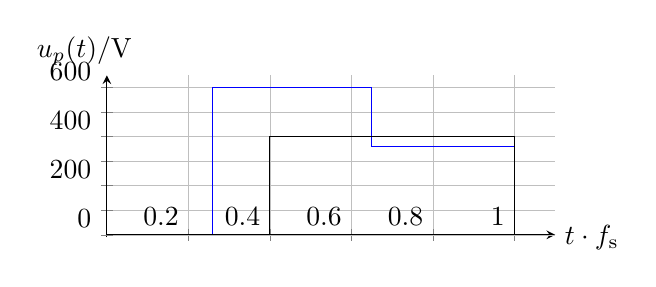
\begin{tikzpicture}
        \begin{axis}[
                domain=0:15,
                % x/y range adjustment
                xmin=0, xmax=1.1,
                ymin=-10, ymax=650,
                samples=200,
                axis y line=center,
                axis x line=middle,
                extra y ticks=0,
                % Label text
                xlabel={$t \cdot f_\mathrm{s}$},,
                ylabel={$u_\text{p}(t)/\mathrm{V}$},
                % Label adjustment
                x label style={at={(axis description cs:1,0)},anchor=west},
                y label style={at={(axis description cs:-.05,1)},anchor=south},
                width=0.6\textwidth,
                height=0.3\textwidth,
                % x-Ticks
                xtick={0,0.2,0.4,0.6,0.8,1},
                xticklabels={0,0.2,0.4,0.6,0.8,1},
                xticklabel style = {yshift=0.3cm,anchor=east},
                % y-Ticks
                ytick={600,500,400,300,200,100,0},
                yticklabels={600,,400,,200,,0},
                yticklabel style = {yshift=0.2cm,anchor=east},
                % Grid layout
                grid=both,
                grid style={line width=.1pt, draw=gray!10},
                major grid style={line width=.2pt,draw=gray!50},
            ]
            %Ut at U1=360V
            \addplot[color=blue,mark=none,solid] coordinates{
                (0, 0)
                (0.26, 0)
                (0.26, 600)
                (0.65, 600)
                (0.65, 360)
                (1,  360)
                (1,0)
                (1.05,0)
                };                
            %Ut at U1=240V
            \addplot[color=black,mark=none,solid] coordinates{
                (0, 0)
                (0.4, 0)
                (0.4, 400)
                (1,  400)
                (1,0)
                (1.05,0)
                };                
            \end{axis}     
    \end{tikzpicture}
    \caption{Voltage at transistor.}
    \label{fig:ex04_VoltageAtTransistor}
    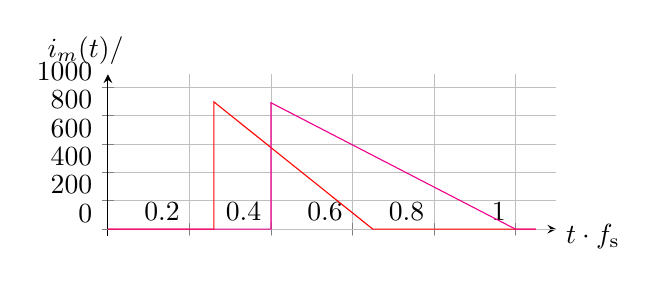
\begin{tikzpicture}
        \begin{axis}[
                domain=0:15,
                % x/y range adjustment
                xmin=0, xmax=1.1,
                ymin=-50, ymax=1090,
                samples=200,
                axis y line=center,
                axis x line=middle,
                extra y ticks=0,
                % Label text
                xlabel={$t \cdot f_\mathrm{s}$},,
                ylabel={$i_\text{m}(t)/\SI{}{\milli\ampere}$},
                % Label adjustment
                x label style={at={(axis description cs:1,0)},anchor=west},
                y label style={at={(axis description cs:-.05,1)},anchor=south},
                width=0.6\textwidth,
                height=0.3\textwidth,
                % x-Ticks
                xtick={0,0.2,0.4,0.6,0.8,1},
                xticklabels={0,0.2,0.4,0.6,0.8,1},
                xticklabel style = {yshift=0.3cm,anchor=east},
                % y-Ticks
                ytick={1000,800,600,400,200,0},
                yticklabels={1000,800,600,400,200,0},
                yticklabel style = {yshift=0.2cm,anchor=east},
                % Grid layout
                grid=both,
                grid style={line width=.1pt, draw=gray!10},
                major grid style={line width=.2pt,draw=gray!50},
            ]
            %im at U1=360V
            \addplot[color=red,mark=none,solid] coordinates{
                (0, 0)
                (0.26, 0)
                (0.26, 896)
                (0.65, 0)
                (1.05,0)
                };                
            %Ut at U1=240V
            \addplot[color=magenta,mark=none,solid] coordinates{
                (0, 0)
                (0.4, 0)
                (0.4, 890)
                (1,0)
                (1,0)
                (1.05,0)
                };                
            \end{axis}     
    \end{tikzpicture}
    \caption{Demagnetization current of  $N_3$.}
    \label{fig:ex04_DemagnetizationCurrentN3}
\end{solutionfigure}




